\documentclass[11pt]{article}
\usepackage{color} %used for font color
\usepackage{amssymb} %maths
\usepackage{amsmath} %maths
\usepackage{bm}
\usepackage{epsfig}
\usepackage{soul}
\usepackage{subcaption}
\usepackage{listings}
\usepackage{authblk}
\usepackage{float}
\usepackage{graphicx}
\usepackage{multicol}
\usepackage{lipsum}
\topmargin-.5in
\textwidth6.6in
\textheight9in
\setlength{\columnsep}{0.6cm}
\oddsidemargin0in
\setlength\parindent{0pt}

%\def\fs{\scriptsize}
\usepackage{listings}
\usepackage{xcolor}

\DeclareMathOperator*{\E}{\mathbb{E}}

%New colors defined below
\definecolor{codegreen}{rgb}{0,0.6,0}
\definecolor{codegray}{rgb}{0.5,0.5,0.5}
\definecolor{codepurple}{rgb}{0.58,0,0.82}
\definecolor{backcolour}{rgb}{0.95,0.95,0.92}

%Code listing style named "mystyle"
\lstdefinestyle{mystyle}{
  backgroundcolor=\color{backcolour},   commentstyle=\color{codegreen},
  keywordstyle=\color{magenta},
  numberstyle=\tiny\color{codegray},
  stringstyle=\color{codepurple},
  basicstyle=\ttfamily\footnotesize,
  breakatwhitespace=false,         
  breaklines=true,                 
  captionpos=b,                    
  keepspaces=true,                 
  numbers=left,                    
  numbersep=5pt,                  
  showspaces=false,                
  showstringspaces=false,
  showtabs=false,                  
  tabsize=2
}

%"mystyle" code listing set
\lstset{style=mystyle}

\title{ \bf{Assignment IV \\ MA797: Special Topics in Machine Learning}}
\author{Alp Tezbasaran$^{a}$}
\affil{\textit{$^{a}$Department of Nuclear Engineering NCSU, alptezbasaran@ncsu.edu}}
\date{November 8, 2019}
\begin{document}
\maketitle

\section{Conversion of mnistcnn.py}

The task is to convert \emph{mnistcnn.py} code to use high-level Tensorflow API, KERAS. For this, first the structure of the model is investigated. The code has the following neural network structure.\medskip


\begin{enumerate}
    \item 1st Convolution layer
    \begin{itemize}
        \item 32 filters
        \item 5x5 filter size
        \item Relu activation
        \item Same padding
        \item Stride 1
    \end{itemize}
    \item 1st MaxPool layer
    \begin{itemize}
        \item 2x2 blocks
        \item Non-overlapping strides
        \item Same padding
    \end{itemize}
    \item 2nd Convolution layer
    \begin{itemize}
        \item 64 filters
        \item 5x5 filter size
        \item Relu activation
        \item Same padding
        \item Stride 1
    \end{itemize}
    \item 2nd MaxPool layer
    \begin{itemize}
        \item 2x2 blocks
        \item Non-overlapping strides
        \item Same padding
    \end{itemize}
    \item Flattening layer
    \item 1st Fully connected layer
    \begin{itemize}
        \item 128 neurons
        \item Relu activation
    \end{itemize}
    \item 1st Dropout layer
    \begin{itemize}
        \item 0.5 as the dropoupt rate
    \end{itemize}
    \item Output layer
    \begin{itemize}
        \item 10 neurons
        \item Softmax activation
    \end{itemize}
\end{enumerate}

Following python code is the converted version of the \emph{mnistcnn.py} with couple modifications. First one is the dropout rate. Since dropout rate in the example is 0, and we are expected to have a dropout layer, I picked it it to be $50\%$. Second difference is the number of neutrons in the fully connected layer. The example has 1024 neurons in the \emph{Dense} layer, however Dr. Flores specifically stated in the email that I am supposed to use 128 neurons. \medskip

There is one more minor change from the original code which is the \emph{loss} function. The imported data has class direct class labels rather than One-Hot encoded labels. So instead using \emph{categorical\_cross\_entropy}, here \emph{\underline{sparse\_categorical\_crossentropy}} is used as the loss function. Similarly, the accuracy metric is \emph{\underline{sparse\_categorical\_accuracy}}. \medskip

First part of the code is importing related libraries, normalizing the data, and reshaping to a format where Keras can read.\medskip

\begin{lstlisting}[language=Python, basicstyle=\tiny, caption=KERAS Sequential model for mnist classification]

import numpy as np
import tensorflow as tf
import matplotlib.pyplot as plt
import datetime

tf.__version__
tf.random.set_seed(0)

mnist = tf.keras.datasets.mnist
(x_train, y_train), (x_test, y_test) = mnist.load_data()

# Look at images
plt.imshow(x_test[0])

x_train, x_test = x_train / 255.0, x_test / 255.0
x_train = x_train.reshape((x_train.shape[0],x_train.shape[1],x_train.shape[2],1))
x_test = x_test.reshape((x_test.shape[0],x_test.shape[1],x_test.shape[2],1))
#plt.imshow(x_test[0])

#Keras sequential
model = tf.keras.models.Sequential()
# 1. Conv2D
model.add(tf.keras.layers.Conv2D(filters=32, kernel_size=5, padding="same", activation="relu", input_shape=(28,28,1)))
# 2. Maxpool
model.add(tf.keras.layers.MaxPool2D(pool_size=2, strides=2, padding='same'))
# 3. Conv2D
model.add(tf.keras.layers.Conv2D(filters=64, kernel_size=5, padding="same", activation="relu"))
# 4. Maxpool
model.add(tf.keras.layers.MaxPool2D(pool_size=2, strides=2, padding='same'))
# 5. Flatten
model.add(tf.keras.layers.Flatten())
# 6. Dense
model.add(tf.keras.layers.Dense(units=128, activation='relu'))
# 7. Dropout
model.add(tf.keras.layers.Dropout(0.5))
# 8. Output
model.add(tf.keras.layers.Dense(units=10, activation='softmax'))

# Summary
model.summary()

# Compile
model.compile(loss="sparse_categorical_crossentropy",
              optimizer="Adam", metrics=["sparse_categorical_accuracy"])

# Tensorboard
log_dir = 'q1_log'+ datetime.datetime.now().strftime("%Y%m%d-%H%M%S")
tensorboard_callback = tf.keras.callbacks.TensorBoard(log_dir=log_dir, histogram_freq=1, write_graph=True, write_images=True)

# Callbacks
early_stoppping = tf.keras.callbacks.EarlyStopping(patience=5, monitor='val_loss', min_delta=1e-4, verbose=1)
save_checkpoint = tf.keras.callbacks.ModelCheckpoint(filepath='bestq1.h5', save_best_only=True, monitor='val_loss', verbose=1)
reduce_lr       = tf.keras.callbacks.ReduceLROnPlateau(monitor='val_loss', factor=0.2,patience=2, min_lr=1e-2, verbose=1)

# Fit
model.fit(x_train, y_train,batch_size = 50, validation_split = 0.2 ,epochs=5000, callbacks=[tensorboard_callback, early_stoppping, save_checkpoint, reduce_lr])

# Eval
test_loss, test_accuracy = model.evaluate(x_test, y_test)

# Load model
loaded = tf.keras.models.load_model('bestq1.h5')
test_loss, test_accuracy = loaded.evaluate(x_test, y_test, verbose = 0)
\end{lstlisting}

It is noteworthy to emphasize, this code uses Tensorflow version 2.0 where \emph{keras} is a module, rather than a high-level wrapper. \medskip

There are few lines need to be emphasized, namely \emph{callbacks}. Callback are useful functions, that can be applied to a training, which includes, saving the model based on some parameters (frequency, minimum validation loss, etc.), reducing the learning rate if there is plateau in the loss function, stopping the training if there is not any increase in accuracy for some pre-defined consecutive iterations. There are more callback options, but the described ones are used in this study. \medskip

Early stopping criteria checks validation loss of the last 5 iterations and if the difference is smaller than $10^{-4}$ stops the fitting. We are asked to save the model that has the lowest validation loss. This is achieved by employing \emph{ModelCheckpoint} callback function. Here, best model is saved to 'bestq1.h5' file each time validation loss decreases. \medskip

Finally, \emph{TensorBoard} callback is used to track training and validation check and evolution of accuracy and loss values. TensorBoard also has capabilities of plotting the architecture of the network, distributions and histograms of kernels and biases. Here data is logged at each epoch. \medskip

Some unmentioned model parameters are listed below.

\begin{itemize}
    \item 80/20 $\%$ training validation split
    \item Adam optimizer
    \item Batch size = 50
    \item Epochs = 5000, but since early stopping is defined with relatively low difference, training stopped after \bm{$14$} epochs.
\end{itemize}


The following table shows the training, validation and out-of sample testing accuracy values.\medskip

\bgroup
\def\arraystretch{1.5}%  1 is the default, change whatever you need
\begin{table}[H]
\centering
\caption{Accuracy of Convolutional Neural Network trained with Mnist dataset}
\begin{tabular}{|c|c|c|c|}
\hline
            &  Training     &  Validation & Out-of Sample   \\ \hline
Accuracy    &  0.9961       & 0.9917      &  0.994          \\ \hline
\end{tabular}
\label{table:q1acc}
\end{table}
\egroup

\section{New Architecture}

This problem asks us to modify the architecture of the convolutional neural network defined in the previous section. The batch normalization layers are to be applied after each convolution layers, with filters kernel size 3x3 and stride of 1.Following list summarizes the layers.


\begin{enumerate}
    \item 1st Convolution layer
    \begin{itemize}
        \item 32 filters
        \item 3x3 filter size
        \item Relu activation
        \item Same padding
        \item Stride 1
    \end{itemize}
    \item 1st Batch Normalization
    \item 1st MaxPool layer
    \begin{itemize}
        \item 2x2 blocks
        \item Non-overlapping strides
        \item Same padding
    \end{itemize}
    \item 2nd Convolution layer
    \begin{itemize}
        \item 32 filters
        \item 3x3 filter size
        \item Relu activation
        \item Same padding
        \item Stride 1
    \end{itemize}
    \item 2nd Batch Normalization
    \item 2nd MaxPool layer
    \begin{itemize}
        \item 2x2 blocks
        \item Non-overlapping strides
        \item Same padding
    \end{itemize}
    \item Flattening layer
    \item 1st Fully connected layer
    \begin{itemize}
        \item 128 neurons
        \item Relu activation
    \end{itemize}
    \item 1st Dropout layer
    \begin{itemize}
        \item 0.5 as the dropoupt rate
    \end{itemize}
    \item Output layer
    \begin{itemize}
        \item 10 neurons
        \item Softmax activation
    \end{itemize}
\end{enumerate}

The other parameters are the same for this model like \emph{Adam} optimizer, 80/20 $\%$ training and validation split, normalization of data, and loss and accuracy definitions. Here number of epochs are defined as 5000 but early stopping is called and the training converged after \bm{$13$} iterations. 

The following table shows the training, validation and out-of sample testing accuracy values.\medskip

\bgroup
\def\arraystretch{1.5}%  1 is the default, change whatever you need
\begin{table}[H]
\centering
\caption{Accuracy of Modified Convolutional Neural Network trained with Mnist dataset}
\begin{tabular}{|c|c|c|c|}
\hline
            &  Training     &  Validation & Out-of Sample   \\ \hline
Accuracy    &  0.9919       & 0.9893      &  0.9886         \\ \hline
\end{tabular}
\label{table:q1acc}
\end{table}
\egroup

Following figures shows the evolution of training and validation loss and accuracy. The plots are generated using TensorBoard.

\begin{figure}[H]
\centering
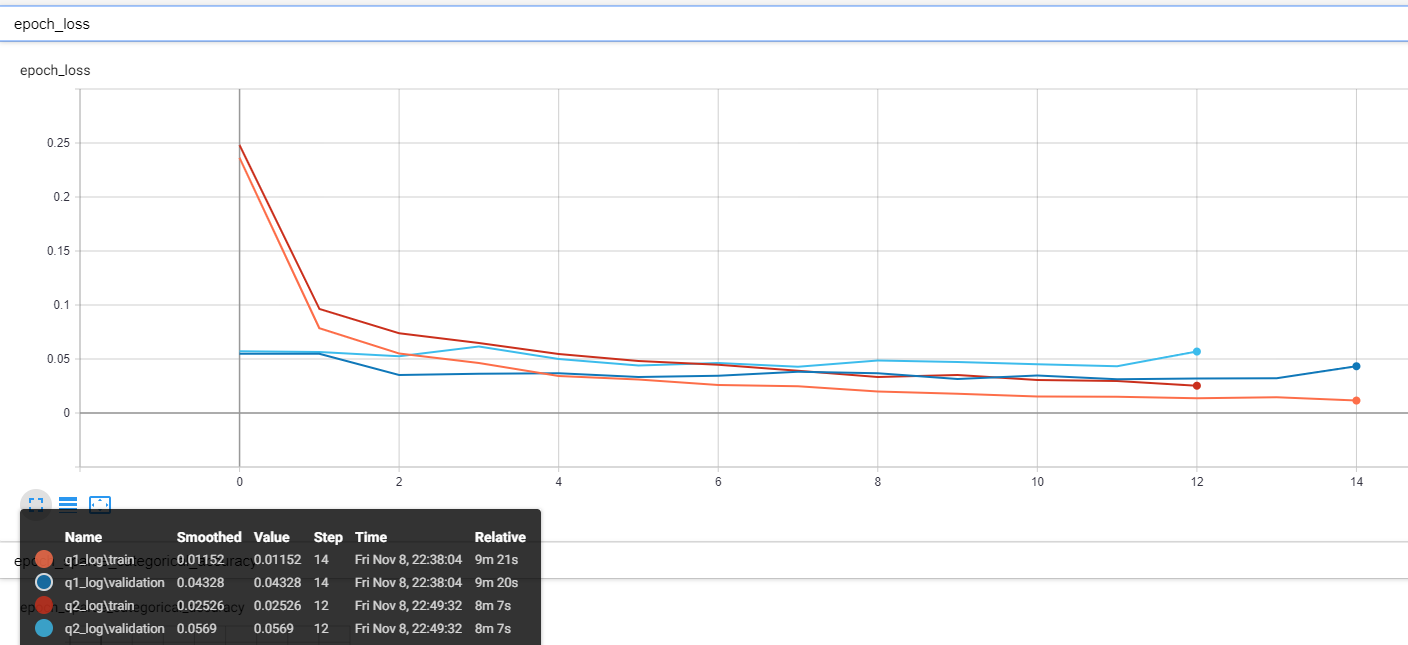
\includegraphics[width=0.95\columnwidth]{pics/epoch_loss.png}
\captionsetup{justification=centering}
\caption{Sparse Categorical Crossentropy Loss vs Epoch}
\label{fig:data}
\end{figure}

\begin{figure}[H]
\centering
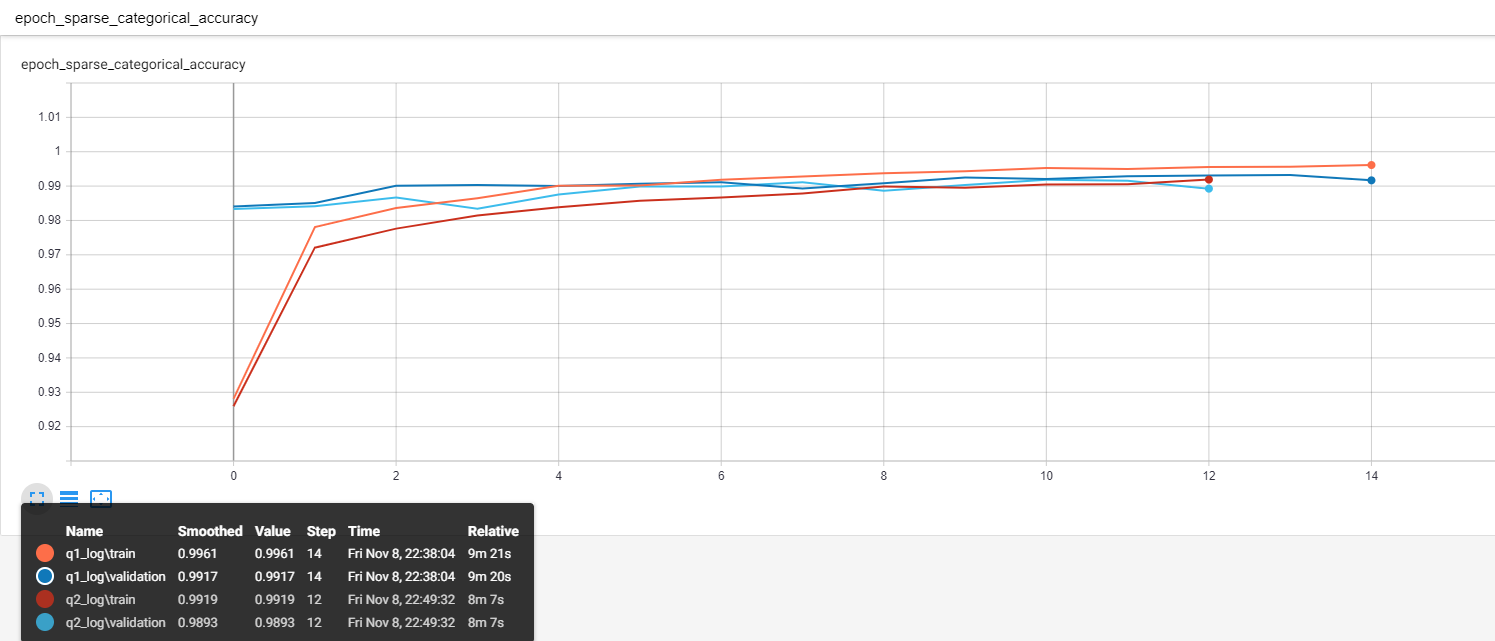
\includegraphics[width=0.95\columnwidth]{pics/epoch_acc.png}
\captionsetup{justification=centering}
\caption{Sparse Categorical Accuracy vs Epoch}
\label{fig:data}
\end{figure}

The code to train the Keras sequential model is shown below

\begin{lstlisting}[language=Python, basicstyle=\tiny, caption=Modified CNN architecture with KERAS Sequential model for mnist classification]
import numpy as np
import tensorflow as tf
import matplotlib.pyplot as plt
import datetime

tf.__version__
tf.random.set_seed(0)

# Import dataset
mnist = tf.keras.datasets.mnist
(x_train, y_train), (x_test, y_test) = mnist.load_data()

# Normalize and reshape
x_train, x_test = x_train / 255.0, x_test / 255.0
x_train = x_train.reshape((x_train.shape[0],x_train.shape[1],x_train.shape[2],1))
x_test = x_test.reshape((x_test.shape[0],x_test.shape[1],x_test.shape[2],1))

#Keras sequential
model = tf.keras.models.Sequential()
# 1. Conv2D - 1
model.add(tf.keras.layers.Conv2D(filters=32, kernel_size=3, padding="same", activation="relu", input_shape=(28,28,1)))
# 2. BatchNorm - 1
model.add(tf.keras.layers.BatchNormalization())
# 3. Maxpool - 1
model.add(tf.keras.layers.MaxPool2D(pool_size=2, strides=2, padding='same'))
# 4. Conv2D - 2
model.add(tf.keras.layers.Conv2D(filters=32, kernel_size=3, padding="same", activation="relu"))
# 5. BatchNorm - 2
model.add(tf.keras.layers.BatchNormalization())
# 6. Maxpool -2
model.add(tf.keras.layers.MaxPool2D(pool_size=2, strides=2, padding='same'))
# 7. Flatten - 1
model.add(tf.keras.layers.Flatten())
# 8. Dense - 1
model.add(tf.keras.layers.Dense(units=128, activation='relu'))
# 9. Dropout - 1
model.add(tf.keras.layers.Dropout(0.5))
#10. Output - 1
model.add(tf.keras.layers.Dense(units=10, activation='softmax'))

# Summary
model.summary()

# Compile
model.compile(loss="sparse_categorical_crossentropy", optimizer="Adam", metrics=["sparse_categorical_accuracy"])

# Tensorboard
log_dir = 'q2_log'+ datetime.datetime.now().strftime("%Y%m%d-%H%M%S")
tensorboard_callback = tf.keras.callbacks.TensorBoard(log_dir=log_dir, histogram_freq=1, write_graph=True, write_images=True)

# Callbacks
early_stoppping = tf.keras.callbacks.EarlyStopping(patience=5, monitor='val_loss', min_delta=1e-4, verbose=1)
save_checkpoint = tf.keras.callbacks.ModelCheckpoint(filepath='bestq2.h5', save_best_only=True, monitor='val_loss', verbose=1)
reduce_lr       = tf.keras.callbacks.ReduceLROnPlateau(monitor='val_loss', factor=0.2,patience=2, min_lr=1e-2, verbose=1)

# Fit
model.fit(x_train, y_train,batch_size = 50, validation_split = 0.2 ,epochs=5000, callbacks=[tensorboard_callback, early_stoppping, save_checkpoint, reduce_lr])

# Eval
test_loss, test_accuracy = model.evaluate(x_test, y_test)

# Load model
loaded = tf.keras.models.load_model('bestq2.h5')
test_loss, test_accuracy = loaded.evaluate(x_test, y_test, verbose = 0)
\end{lstlisting}

The following screenshot shows options to generate the plots above.

\begin{figure}[H]
\centering
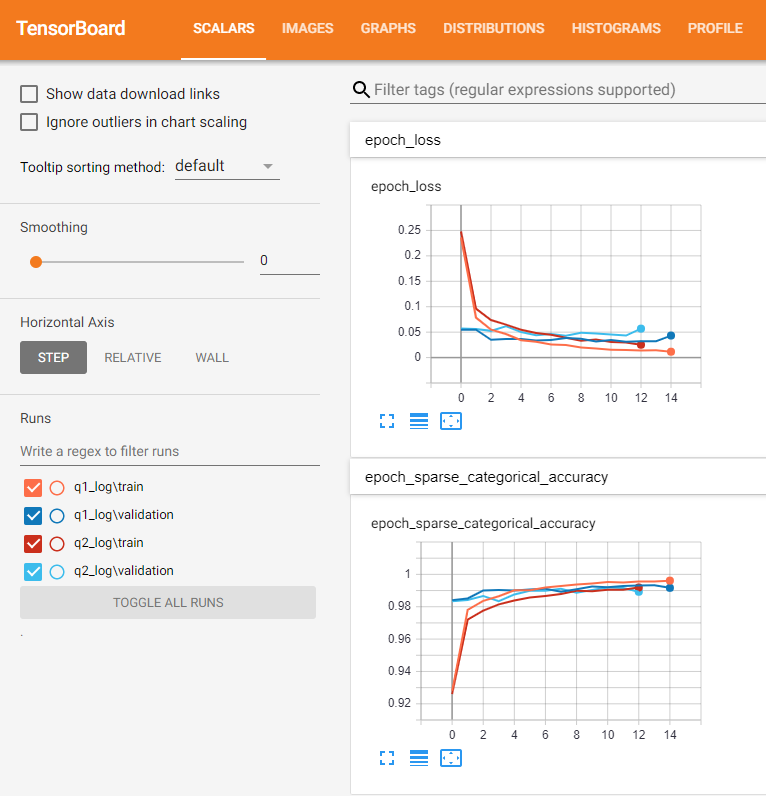
\includegraphics[width=0.65\columnwidth]{pics/tb2.png}
\captionsetup{justification=centering}
\caption{TensorBoard Scalars screen}
\label{fig:data}
\end{figure}

\end{document}
